% include the figures path relative to the master file
\graphicspath{ {./content/intro/figure/} }

\section{Introduction}

Active infrared thermography becomes one of the essential techniques for \ac{ndt}. Approaches like \ac{pt}\cite{Maldague2002} \ac{ppt} \cite{Maldague1996} or \ac{lt} \cite{Wu1998} have proved to be effective to characterize defects. 
In recent years, an evolution of NDT systems by adding 3D measurement can be noted. Fernandes et al.\cite{fernandes2015fiber} reconstruct carbon fiber objects using 3D scanner and determine the orientation of the fiber with a laser and an infrared camera. Subsequently, the thermal information is mapped to the reconstructed 3D model. Similarly, Oswald-Tranta et al.\cite{Oswald-Tranta2012} detect crack in non-magnetic materials based on the fusion between the infrared and the 3D data, obtained through an inductive \ac{ndt}system and a conventional stereo vision system, respectively.
To quantify the energy losses in buildings, Vidas et al.\cite{Vidas2013} map the thermal information on the 3D data using a Microsoft Kinect and a thermal camera. To conclude, it can be noted that most of the proposed prototypes are actually using two systems: a 3D scanner and a non-destructive inspection system in the infrared range. These hybrid systems in which distinct steps of 3D reconstruction and \ac{ndt} inspection suffer from drawback such as errors during the data fusion.

\begin{figure}
  \centering
  \hspace*{\fill}
  \subfigure[]{\label{subfig:1a}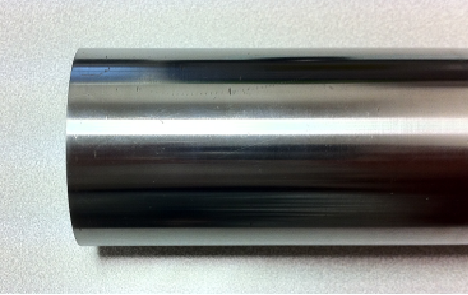
\includegraphics[width=0.15\linewidth]{A1.png}} \hfill
  \subfigure[]{\label{subfig:1b}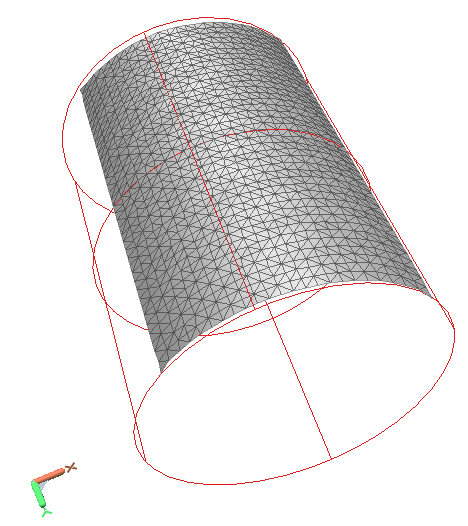
\includegraphics[width=0.15\linewidth]{A2.png}} \hfill
  \subfigure[]{\label{subfig:1c}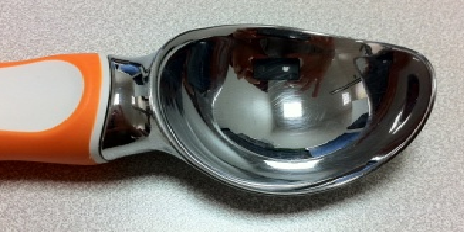
\includegraphics[width=0.15\linewidth]{B1.png}} \hfill
  \subfigure[]{\label{subfig:1d}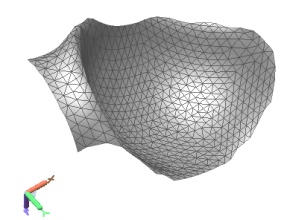
\includegraphics[width=0.15\linewidth]{B2.png}}
  \hspace*{\fill} \\ \hspace*{\fill}
  \subfigure[]{\label{subfig:1e}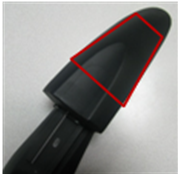
\includegraphics[width=0.15\linewidth]{C1.png}} \hfill
  \subfigure[]{\label{subfig:1f}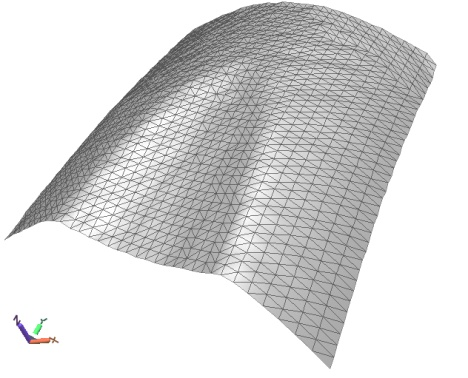
\includegraphics[width=0.15\linewidth]{C2.png}} \hfill
  \subfigure[]{\label{subfig:1g}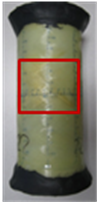
\includegraphics[width=0.1\linewidth]{D1.png}} \hfill
  \subfigure[]{\label{subfig:1h}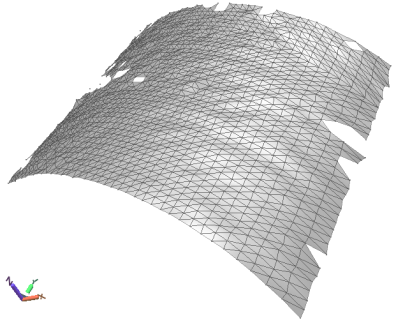
\includegraphics[width=0.15\linewidth]{D2.png}}
  \hspace*{\fill} \\ \hspace*{\fill}
  \subfigure[]{\label{subfig:1i}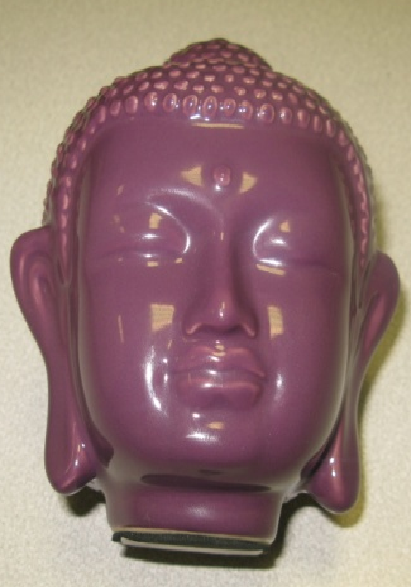
\includegraphics[width=0.15\linewidth]{E1.png}} \hfill
  \subfigure[]{\label{subfig:1j}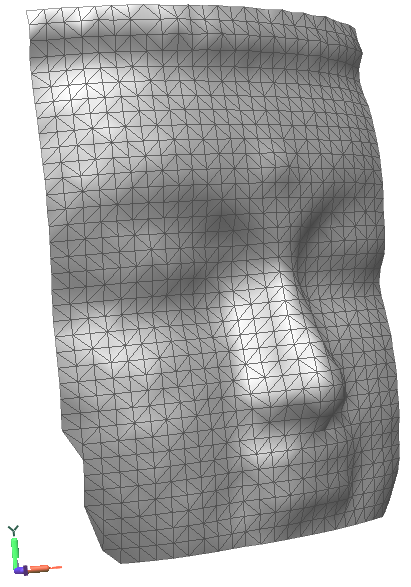
\includegraphics[width=0.15\linewidth]{E2.png}} \hfill
  \subfigure[]{\label{subfig:1k}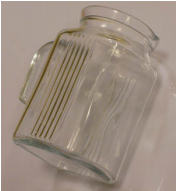
\includegraphics[width=0.15\linewidth]{F1.png}} \hfill
  \subfigure[]{\label{subfig:1l}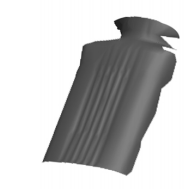
\includegraphics[width=0.15\linewidth]{F2.png}}
  \hspace*{\fill}
  \caption{Examples of 3D digitization obtained by \acs*{sfh} approach: (a), (b), (c) and (d) metallic specular surfaces \cite{bajard2013numerisation} - (e) and (f) black plastic - (g) and (h) composite material - (i) and (j) ceramic - (k) and (l) glass transparent object \cite{meriaudeau20113d}.}
  \label{fig:1}
\end{figure}

% \begin{figure}
%   \centering
%   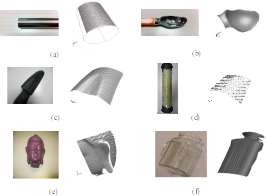
\includegraphics[width=0.7\linewidth]{fig1.png}
%   \caption{Examples of 3D digitization obtained by \acs*{sfh} approach: (a) and (b) metallic specular surfaces (c) black plastic, (d) composite material, (e) ceramic and (f) glass transparent object.}
%   \label{fig:1}
% \end{figure}

\ac{sfh} offers an alternative. This approach is initially used to reconstruct objects into 3D. Indeed, Eren et al.\cite{Eren2009} achieve impressive results using \ac{sfh} in which the geometry of glass or plastic transparent objects is estimated based on active triangulation. The transparent object placed on a gliding stage is locally heated using a CO2 laser source of \SI{10.6}{\micro \metre} wavelength. The emitted radiation is acquired by an Infra-Red (IR) camera and the 3D position of the heated point is recovered thanks to a prior calibration, with an accuracy in the order of \SI{100}{\micro \metre}.

Bajard et al.\cite{Bajard2012} have extended this method for metal objects which have different radiative and conductive properties. The CO2 laser source is replaced by an Nd~:YAG Laser of \SI{1.06}{\micro \metre} wavelength, since the metals absorption coefficient is 4 times greater at \SI{1.06}{\micro \metre} than at \SI{10.6}{\micro \metre}. The results of the specular objects digitization are shown in Fig.\,\ref{fig:1}. Other examples of 3D reconstruction are presented for black plastic, composite material, and ceramic using the same system.

In this work, we present an approach in which \ac{sfh} is extended to perform both 3D reconstruction and \ac{ndt}. We aim at detecting non-through defect and estimate the orientation of fibers using punctual stimulation. The proposed approach significantly reduces the cost of the hardware setup and avoids data fusion errors. Furthermore, a simulation is carried out to demonstrate that the non-defective area can be localized using the thermal radiation disturbance.

The rest of the paper is organized as follows: Section~\ref{sec:2} summarizes related works regarding \ac{ndt} based on punctual stimulation. The proposed method is explained in Sect.\,\ref{sec:3} while Sect.\,\ref{sec:4} presents experimental results. Conclusion and avenues for future directions are drawn in Sect.\,\ref{sec:5}.


% Some stuff that emac's colleagues use
%%% Local Variables:
%%% mode: late
%%% TeX-master: "../../master.tex"
%%% End: \section{introduction}

